\section{Electronic Component Selection} \label{sec:electronic}

The main constraints of the hardware selection is the power consumption, communication capability, network performance and software support. We have done research about the microprocessors and we decided to buy raspberry pi zero w since this model has WiFi built in, but it was out of stock in the markets in Turkey. Therefore, we decided to buy raspberry pi zero wh which can be seen in the figure \ref{fig:raspberry pi zero wh}. We also decided to buy camera module that has 5mp resolution and supports 1080p video capturing as seen in the figure \ref{fig:raspberry pi camera module}. Furthermore, we decided to buy 16gb microsd card. We also did research about voltage regulators, audio opamps and 555timer opamps.

\begin{figure}[h]
    \centering
    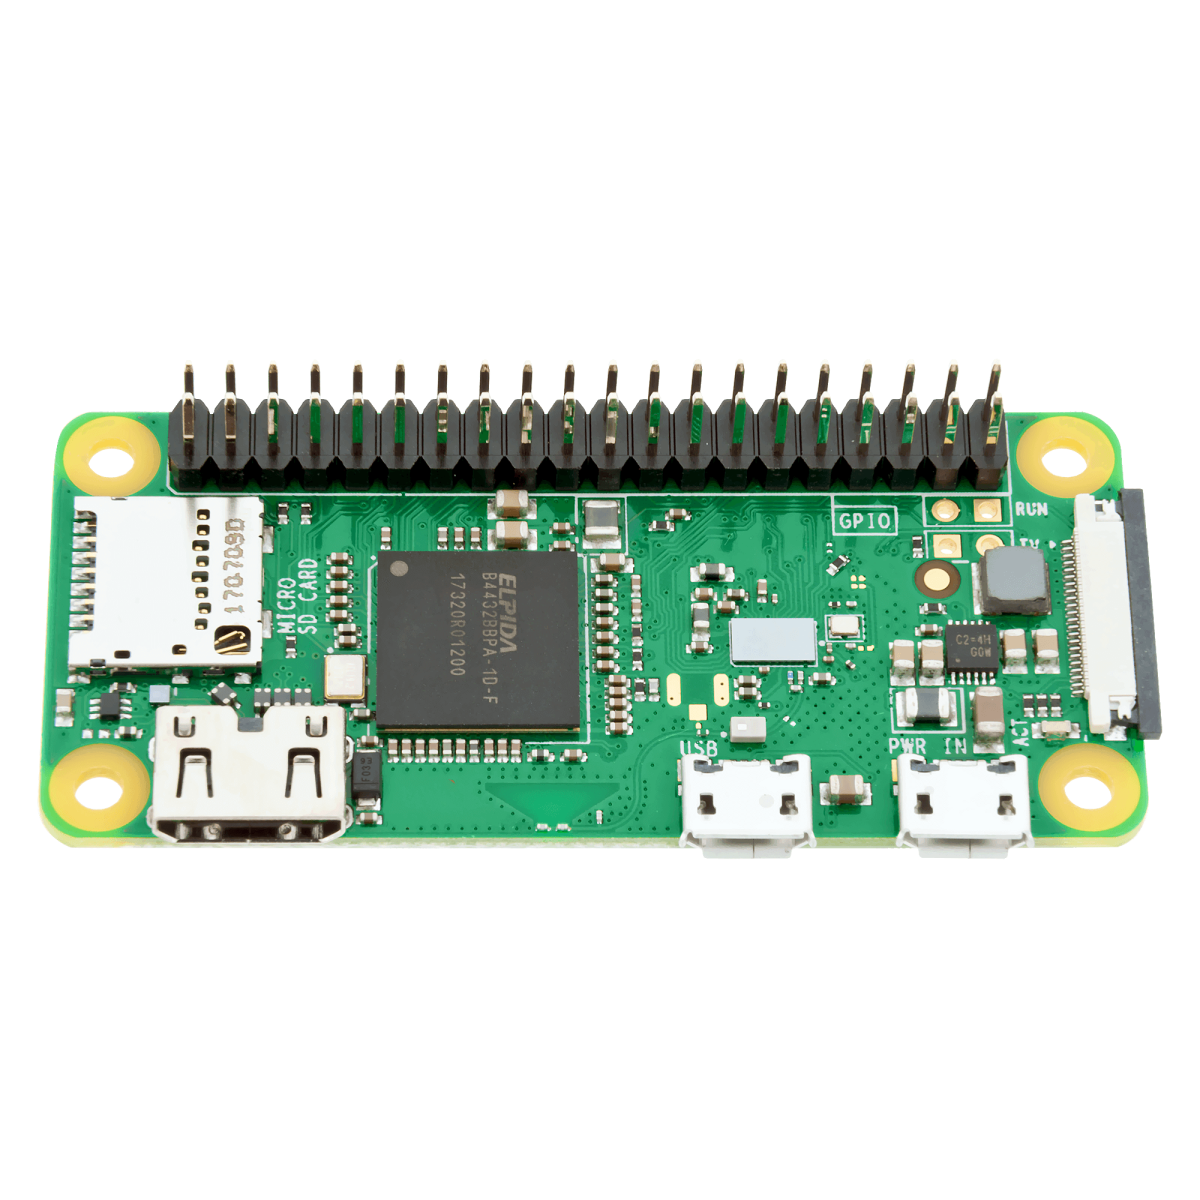
\includegraphics[width=.35\linewidth]{img/pizerowh.png}
    \caption{raspberry pi zero wh}
    \label{fig:raspberry pi zero wh}
\end{figure}

\begin{figure}[b]
    \centering
    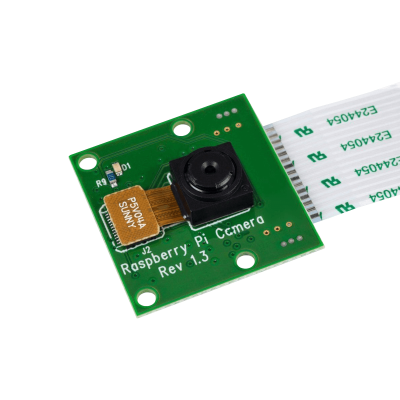
\includegraphics[width=.35\linewidth]{img/picammodule.png}
    \caption{raspberry pi camera module}
    \label{fig:raspberry pi camera module}
\end{figure}





